\chapter{The Arithmetic of Durable Wealth}

In this School of Hard Knocks interview, curated by LazyingArt LLC, the mathematics arrives without a blackboard. It comes instead as a sequence of operational recursions. We are first shown scale, then asked about debt, then led through cash-funded asset accumulation, then through the copying of measured operations, and finally through the reserve logic required by volatile income. Because no validated mathematical frame survives from this lecture, every displayed formula and every figure below is either transcript-backed or a cautious reconstruction of spoken reasoning. The safest way to read the lecture is to keep its order. The order is part of the proof.

\section{Scale First, Explanation Second}

The host opens by stacking magnitude before doctrine. We hear that Ramsey made hundreds of millions in a single year, that Jimmy John's sale ran into the billions, and that Charlie Sheen belongs to the class of actors whose earnings became part of television folklore. This is not yet analysis. It is scale-establishment. The lecture wants us to feel the size of the objects before it tells us how those objects were made.

The cleanest markers are
\begin{align}
R_{\mathrm{Ramsey}} &\approx \$300\,\mathrm{M/yr},\\
V_{\mathrm{campus}} &\approx \$650\,\mathrm{M},\\
V_{\mathrm{RE}} &\approx \$850\,\mathrm{M},\\
V_{\mathrm{Jimmy}} &\approx \$3.5\,\mathrm{B}.
\end{align}
Already the lecture is teaching us to separate kinds of quantity. Revenue is not valuation. Campus value is not the same as total real-estate value. Sale price is not annual operating cash. The opening sounds noisy, but the bookkeeping problem is real: what sort of number are we even looking at?

Charlie Sheen's presence sharpens the point. There the host does not begin with a balance sheet. He begins with celebrity scale and with the memory of extreme compensation. The lecture is therefore not yet asking only how to build a business. It is asking a wider question: what structures make large wealth durable, and what happens when the surrounding conditions are unstable?

Only after that overload of scale do we arrive at Dave Ramsey's campus, where the first serious mechanism is finally put on the table.

\section{Ramsey's Anti-Debt Theorem in Interview Form}

At Ramsey's headquarters the host does two things in quick succession. He points at the campus and he asks the question that makes the whole section move: if giant firms borrow, why refuse debt? Ramsey answers first with category discipline and then with principle. The campus itself is said to be about \( \$650\,\mathrm{M}\); the broader real-estate holding is said to be about \( \$850\,\mathrm{M}\); and it is all cash.

Ramsey then compresses his doctrine into the sentence \emph{debt equals risk}. We should not read that as an exact identity. We should read it as the sign of the model:
\begin{equation}
\frac{\partial F}{\partial D}>0,
\end{equation}
where \(D\) is debt and \(F\) is fragility under shock. In a slightly more explicit form, the same idea is
\begin{equation}
DS>0 \ \land\ R_t\downarrow \ \Rightarrow\ P(\text{distress})\uparrow,
\end{equation}
with \(DS\) denoting debt service and \(R_t\) the revenue stream. Debt creates a fixed claim. A fixed claim is most dangerous precisely when revenue is least cooperative.

\paragraph{Anecdote.} The host's objection is the right one. Apple borrows. The biggest companies borrow. Why not take the extra capital and scale faster?

\paragraph{Claim.} Ramsey's answer is categorical: no borrowing at all, ever, for anything.

\paragraph{Mechanism.} Organic cash growth is slower, but it removes the fixed claim that can turn a bad revenue period into a fatal one. The COVID example is the lecture's stress test. The firm with no debt may still suffer. It need not be pushed into insolvency by covenant and payment schedule.

\subsection{Question \& Answer}

\paragraph{Question.} If the biggest companies borrow, why refuse debt entirely?

\paragraph{Answer.} Because the lecture's standard of success is not maximum speed but lower fragility. Borrowing can buy growth, but it also installs a non-negotiable claimant in the capital structure. Ramsey is willing to grow more slowly in exchange for a business that does not become mechanically endangered when revenue is interrupted. In the lecture's own practical spirit, the rule can be summarized as
\begin{equation}
DS=0 \ \Rightarrow\ P(\text{insolvency}\mid R_t\downarrow)\ \text{is reduced}.
\end{equation}
This is not a full bankruptcy theory. It is a selection rule about what kinds of risks we are willing to own.

\section{Cash-Funded Real Estate and the Positive Snowball}

Once the refusal of debt is stated, the host immediately presses on the real obstacle. If we do not borrow, how do we buy anything large? Ramsey's answer is not glamorous. It is sequential. Buy what you can buy. Wait where you must wait. Reinvest what the operating business throws off.

The first land purchase is unusually concrete:
\begin{equation}
P_0=\$10\,\mathrm{M},\qquad A_0=48\ \text{acres}.
\end{equation}
What matters here is not only the price or acreage. What matters is the phrase ``we just bought the dirt.'' The land was acquired before the money existed to do anything elaborate with it. The lecture is insisting that ownership of the site can come first and full development later.

The underlying cash loop may be written, cautiously, as
\begin{equation}
K_{t+1}=K_t+CF_t-C_{\mathrm{draw},t}-I_t,
\end{equation}
where \(K_t\) is liquid retained capital, \(CF_t\) is operating cash flow, \(C_{\mathrm{draw},t}\) is cash removed from the business, and \(I_t\) is the capital committed to land and buildings. That formula is not spoken verbatim, but it is exactly the structure licensed by Ramsey's own description: save, watch the cash flow, and keep putting what the firm makes into ``this concrete thing here.''

\begin{figure}[h]
\centering
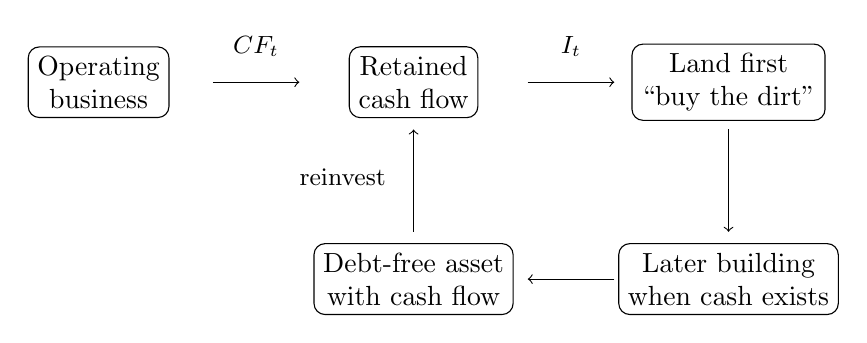
\begin{tikzpicture}[scale=1]
\node[draw, rounded corners, align=center] (op) at (0,0) {Operating\\business};
\node[draw, rounded corners, align=center] (cf) at (4,0) {Retained\\cash flow};
\node[draw, rounded corners, align=center] (land) at (8,0) {Land first\\``buy the dirt''};
\node[draw, rounded corners, align=center] (build) at (8,-2.5) {Later building\\when cash exists};
\node[draw, rounded corners, align=center] (asset) at (4,-2.5) {Debt-free asset\\with cash flow};

\draw[->] (1.45,0) -- (2.55,0);
\draw[->] (5.45,0) -- (6.55,0);
\draw[->] (8,-0.6) -- (8,-1.9);
\draw[->] (6.55,-2.5) -- (5.45,-2.5);
\draw[->] (4,-1.9) -- (4,-0.6);

\node at (2,0.45) {\small \(CF_t\)};
\node at (6,0.45) {\small \(I_t\)};
\node at (3.1,-1.2) {\small reinvest};
\end{tikzpicture}
\caption{Transcript-based reconstruction of Ramsey's cash-funded capital loop.}
\end{figure}

The lecture then adds the second ingredient: patience under market dislocation. Ramsey says that in 2008 he was buying good property at roughly \(15\%\) to \(20\%\) on the dollar:
\begin{equation}
P_{\mathrm{buy}} \approx (0.15\text{--}0.20)\,P_{\mathrm{former}}.
\end{equation}
A simple numerical example makes the point clear. If a property had once sold for
\[
P_{\mathrm{former}}=\$10\,\mathrm{M},
\]
then the crisis acquisition range would be
\begin{align}
P_{\mathrm{buy,low}} &\approx 0.15\,P_{\mathrm{former}}=\$1.5\,\mathrm{M},\\
P_{\mathrm{buy,high}} &\approx 0.20\,P_{\mathrm{former}}=\$2.0\,\mathrm{M}.
\end{align}
The lecture is not claiming a universal law of real-estate pricing. It is showing what cash and patience can do when the market is under stress.

From there the ``positive snowball'' becomes intelligible. Debt-free properties throw off cash. That cash can help fund the next acquisition. If \(E_{n+1}\) is the equity needed for property \(n+1\), then the condition for the next step is simply
\begin{equation}
\sum_{i=1}^{n}\sum_{t=0}^{T-1} CF_t^{(i)} \ge E_{n+1}.
\end{equation}
That is why the spoken ordering matters so much. The first property is hardest. The second is next hardest. The third is next hardest. Only after that does the snowball begin to feel like a snowball.

\subsection{Question \& Answer}

\paragraph{Question.} How do we buy large real estate without borrowing?

\paragraph{Answer.} We do not leap to the finished building. We control the land, defer the expensive part, let the operating business generate cash, and retain that cash long enough for it to become deployable capital. Then, when crisis discounts appear, cash gives us an advantage that leverage cannot. Ramsey's anti-debt rule is therefore not passive caution. It is a way of preserving optionality for the moment when markets misprice valuable assets.

\section{From No Rescue to No Easy Button}

At this point the lecture could have remained a narrow tract on leverage and property. It does not. It widens into a theory of tempo. Nobody is coming to discover us. Nobody is coming to save us. The Lone Ranger is not coming. The cavalry is not coming. The work must be done repeatedly, whether or not the worker feels heroic on that particular day.

The arithmetic of that idea is elementary but important:
\begin{equation}
X_N = X_0 + \sum_{t=0}^{N-1}\delta_t.
\end{equation}
No single \(\delta_t\) needs to be dramatic. Large visible outcomes are often the accumulated result of many small increments: one conversation at a time, one step at a time, one day of leaving the cave and dragging something home.

The generational turn in the interview belongs here, not elsewhere. Ramsey is not saying that younger people lack possibility. In fact he says the opposite: they often possess abundance-mindedness because they grew up with a magic wand in their hand. Push a button and food arrives. Push a button and answers arrive. Push a button and possibility seems immediate. The hidden danger is not scarcity but speed. One begins to look for an easy button. Ramsey's closing image is culinary rather than financial: the best barbecue is cooked all weekend, not in the microwave.

That is the moral extension of the anti-debt argument. The slow path is not merely a balance-sheet preference. It is a whole anthropology of progress.

The host then compresses all of this into a much cleaner slogan: Ramsey ``invested his way to generational wealth.'' The line is not false, but it is too thin. Entrepreneurship, debt refusal, cash retention, staged land acquisition, and patience have all been folded into a softer phrase. The lecture immediately turns that compression into a product, pivoting into a monetized ``Generational Wealth Day'' event. We should not let the advertisement dominate the chapter, but we should keep the interruption. It shows that the series itself repeatedly converts billionaire synthesis into monetized access.

\section{Jimmy John: Measurement, Intelligibility, and Asset Choice}

Jimmy John's entrance changes the texture of the lecture. Ramsey gave us the arithmetic of fragility and patience. Jimmy gives us the arithmetic of replication. The host has already told us the exit number:
\begin{equation}
V_{\mathrm{Jimmy}} \approx \$3.5\,\mathrm{B}.
\end{equation}
But Jimmy narrates the beginning in almost the opposite register. He did not start with a multi-billion-dollar vision. He says, bluntly, that he wanted enough money for beer and weed. He was second to last in his class. The point is not anti-school theater. The point is that credential ranking and entrepreneurial construction are different variables.

The first genuine theorem of his section arrives through Jamie Coulter. We are told the date and the counts:
\begin{equation}
N_{\mathrm{sub},1987}=4,\qquad N_{\mathrm{PizzaHut,mentor}}=25.
\end{equation}
A man who already knows how to scale restaurants tells Jimmy the rule he still remembers decades later:
\begin{equation}
x\ \text{unmeasured} \Rightarrow x\ \text{unmanaged}.
\end{equation}

\paragraph{Anecdote.} The advice does not come as abstract wisdom. It comes from a stronger operator who shares process, procedure, and the habits by which a small chain stops improvising.

\paragraph{Claim.} ``If you can't measure it, you can't manage it. Know your numbers.''

\paragraph{Mechanism.} Once the numbers are visible, procedure can be disciplined. Once procedure is disciplined, it can be copied. And once it can be copied, scale ceases to be accidental.

Jimmy adds a companion maxim: people do what you do, not what you tell them. That line is the human side of the same theorem. Measurement disciplines the system; imitation disciplines the culture.

The interview then turns, naturally, from store procedure to capital placement. Jimmy says he had become a billionaire before the sale because the business was already throwing off money and he saved it. Since he did not think of himself as a sophisticated investor, he bought land, farmland, and gold. The lecture is not celebrating ignorance. It is clarifying the next filter: the asset must be understandable.

\subsection{Question \& Answer}

\paragraph{Question.} What should rich people buy if they do not yet know how to invest?

\paragraph{Answer.} Jimmy's answer is to buy what one can genuinely understand. His test is almost comically severe. He wants to be able to understand the asset on a single sheet of paper and relate to it concretely:
\begin{equation}
I(a)=1 \iff a\ \text{can be understood on one sheet and related to concretely}.
\end{equation}
That is why real estate passes. Farm ground passes. Opaque stories fail.

The farm-ground cycle is then described in the simplest possible terms:
\begin{equation}
\text{land}+\text{inputs}\rightarrow \text{plant}\rightarrow \text{rain risk}\rightarrow \text{harvest}\rightarrow \text{sale}.
\end{equation}
Its simplicity is the reason it qualifies. The lecture is not hunting for maximal novelty. It is hunting for intelligibility.

Finally Jimmy gives the people-filter:
\begin{equation}
E[R\mid q_{\mathrm{operator}}] > E[R\mid \text{asset story alone}].
\end{equation}
He calls this ``bet the jockey, not the horse.'' The inequality is heuristic rather than statistical, but its ranking is clear. Operator quality outranks narrative glamour. Performance outranks excuses.

\section{Jimmy John: Turnaround Mechanics and Delivery Economics}

The interview then turns back from asset choice to the more violent question of operational rescue. Around 2003, Jimmy says, the system had on the order of
\begin{equation}
N_{\mathrm{stores}}\approx 200,\qquad N_{\mathrm{failing}}\approx 70.
\end{equation}
This is where the lecture might have chosen a miracle story. It does not. Jimmy says the first change was that he quit selling. He began telling the truth.

The truth was that the sandwich business is not casual. It is \(24/7\), \(365\). It is lifestyle-level hard. It is a grind. Even the line ``flavor costs money'' belongs to the mechanics here. Quality is not free, and a business built on freshness has a cost structure that weak operators will underestimate.

The redesign of the franchise machine followed from that honesty. Territories were no longer handed out in broad chunks. Stores were offered one at a time. If the operator handled one well, perhaps more would follow. Jimmy calls this a reverse pitch. The more truthfully he described the hardship, the more serious the applicants became.

The expansion that followed is given in a single large count:
\begin{equation}
N_{\mathrm{later}}\approx 2500.
\end{equation}
The lecture does not attribute that scale to charisma alone. It attributes it to a stricter operator-selection rule and to the willingness to tell people the real cost of creation.

The work-life-balance exchange belongs here too. Jimmy's claim is deliberately harsh: when one is building something out of nothing, ``work-life balance'' is not an available phrase. We should not elevate that to a universal theorem. We should hear it as an operator rule about creation under pressure.

Only then does the lecture arrive at the most elegant business equation in the chapter. The host asks about freaky fast delivery, expecting a branding story. Jimmy answers with location economics. He could not afford A locations. So he took B and C locations, and delivery plus relentless campus sampling let those locations behave like something better:
\begin{equation}
r_{BC}+h_{\mathrm{delivery}} \Rightarrow Q_A.
\end{equation}
Here \(r_{BC}\) is the lower rent of B/C real estate, \(h_{\mathrm{delivery}}\) is delivery hustle plus disciplined off-site sampling, and \(Q_A\) is A-level sales. This is not a slogan. It is arbitrage.

\begin{figure}[h]
\centering
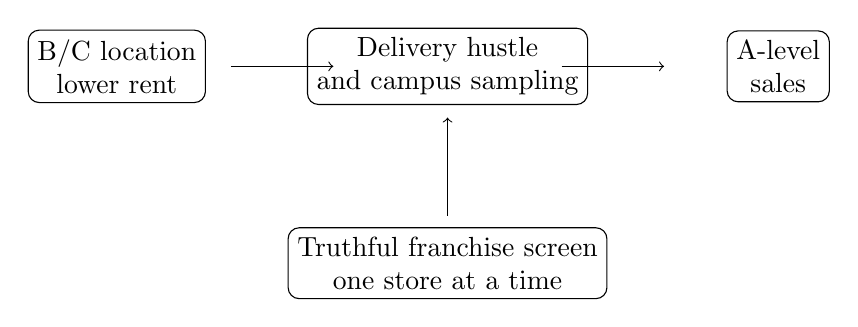
\begin{tikzpicture}[scale=1]
\node[draw, rounded corners, align=center] (rent) at (0,0) {B/C location\\lower rent};
\node[draw, rounded corners, align=center] (delivery) at (4.2,0) {Delivery hustle\\and campus sampling};
\node[draw, rounded corners, align=center] (sales) at (8.4,0) {A-level\\sales};

\draw[->] (1.45,0) -- (2.75,0);
\draw[->] (5.65,0) -- (6.95,0);

\node[draw, rounded corners, align=center] (screen) at (4.2,-2.5) {Truthful franchise screen\\one store at a time};
\draw[->] (4.2,-1.9) -- (4.2,-0.65);
\end{tikzpicture}
\caption{Transcript-based reconstruction of Jimmy John's location arbitrage and franchise-discipline logic.}
\end{figure}

\subsection{Question \& Answer}

\paragraph{Question.} What actually fixed the failing stores, and why did delivery become a decisive edge?

\paragraph{Answer.} The first fix was not cosmetic. Jimmy changed the operator pool by telling the truth about the grind and by allocating stores one at a time. Delivery then solved a different problem. It let weaker real estate participate in stronger revenue by extending the reach of demand. The result was a compound advantage: better operators and cheaper locations made to behave like better ones.

The interview closes this whole section with a different kind of summary. Jimmy says he survived the betrayals, rip-offs, scams, and all the rest. That sentence is not mathematics, but it is part of the model. The machine only compounds if the operator remains alive inside it long enough.

\section{Charlie Sheen as a Volatility Coda}

The final movement changes the regime entirely. The host introduces Charlie Sheen backstage, through legend, notoriety, and the memory of very high pay. This is not a founder with stores and parcels. It is a performer with a spigot.

Charlie begins, interestingly, by disclaiming expertise. That disclaimer is garbled in places, but the financial core that follows is stable and sharp. Never assume the spigot stays open. Sock some away for a rainy day, because the rainy day may become a rainy decade. The clean update rule is therefore
\begin{equation}
S_{t+1}=S_t+Y_t-C_t,
\end{equation}
where \(S_t\) is savings, \(Y_t\) is income, and \(C_t\) is spending. In the language of the interview,
\begin{equation}
Y_t \not\equiv \text{constant} \Rightarrow S_t\ \text{must buffer a multi-period drought}.
\end{equation}
Ramsey gave us resilience against leverage. Charlie gives us resilience against intermittency.

The lecture then widens, as it did with Ramsey, from money to anthropology. Charlie says the driving factor in a highly competitive field was believing in himself when others did not. He talks about risk, about exploring different genres, and about staying open to surprise. People, he says, continue to surprise you. That line matters because volatility here is not merely financial. It is also social and institutional.

The host then turns to the public rises and falls. Charlie's answer is the conceptual identity of the section:
\begin{equation}
\text{industry timeout} \neq \text{self-timeout}.
\end{equation}
Hollywood may banish the person for a period. It does not automatically put the mind into a timeout. That is the inner analogue of reserve capital: something in the self must remain liquid enough to restart.

\subsection{Question \& Answer}

\paragraph{Question.} What do we do when the spigot shuts off?

\paragraph{Answer.} First, we save before it shuts off. That is the direct financial answer. Second, we refuse to let external rejection become inward paralysis. Charlie's next stable claim is that it is never too late to get a fresh start. The section closes with yet another discipline rule, learned from his father: honor the work. That is the deeper recurrence. Save while the income exists. Preserve belief while the institution wavers. Keep faith with the work so that a restart still has a structure to return to.

The final maxim is crude and compressed, but it belongs to the lecture's cadence: do not wreck the thing. By the end, Charlie has supplied not a theory of enterprise scale, but a theory of survival under reputational and income volatility.

\section{Summary}

The lecture begins in spectacle and ends in discipline. What survives the noise is a small family of recursions:
\begin{align}
D\uparrow &\Rightarrow F\uparrow,\\
CF_t\ \text{retained} &\Rightarrow \text{next asset becomes fundable},\\
\text{measurement} &\Rightarrow \text{manageable scale},\\
r_{BC}+h_{\mathrm{delivery}} &\Rightarrow Q_A,\\
Y_t\ \text{volatile} &\Rightarrow S_t\ \text{must exist}.
\end{align}
Ramsey gives us the slow anti-fragile path: pay cash, move slowly, let debt-free assets throw off cash, and do not wait for rescue. Jimmy John gives us the operator's path: know the numbers, buy what is legible, pick performers, tell the truth about the grind, and use delivery to change the geometry of the store. Charlie Sheen gives us the volatility coda: save against dry periods, do not mistake public exile for inward extinction, and honor the work strongly enough that a fresh start remains possible.

The chapter therefore does not reduce to one secret. It gives us a sequence. Scale is shown first. Mechanism appears second. Wealth is built by retention, selection, repetition, and reserves. That is the arithmetic of durable wealth in this lecture.